\documentclass{article}
\usepackage{tikz}

\usetikzlibrary{positioning}
\usetikzlibrary{arrows}
\usetikzlibrary{arrows.meta}

\tikzset{%
	>={Latex[width=2mm,length=2mm]},
	% Specifications for style of nodes:
	base/.style = {rectangle, rounded corners, draw=black, minimum width=4cm, minimum height=1cm, text centered, font=\sffamily},
	input/.style = {base, fill=blue!30},
	process/.style = {base, fill=red!30},
	output/.style = {base, fill=green!30},
}



\title{Pipeline}
\date{09/02/2018}
\author{Irdi Balla}

\begin{document}
	\maketitle	
	
	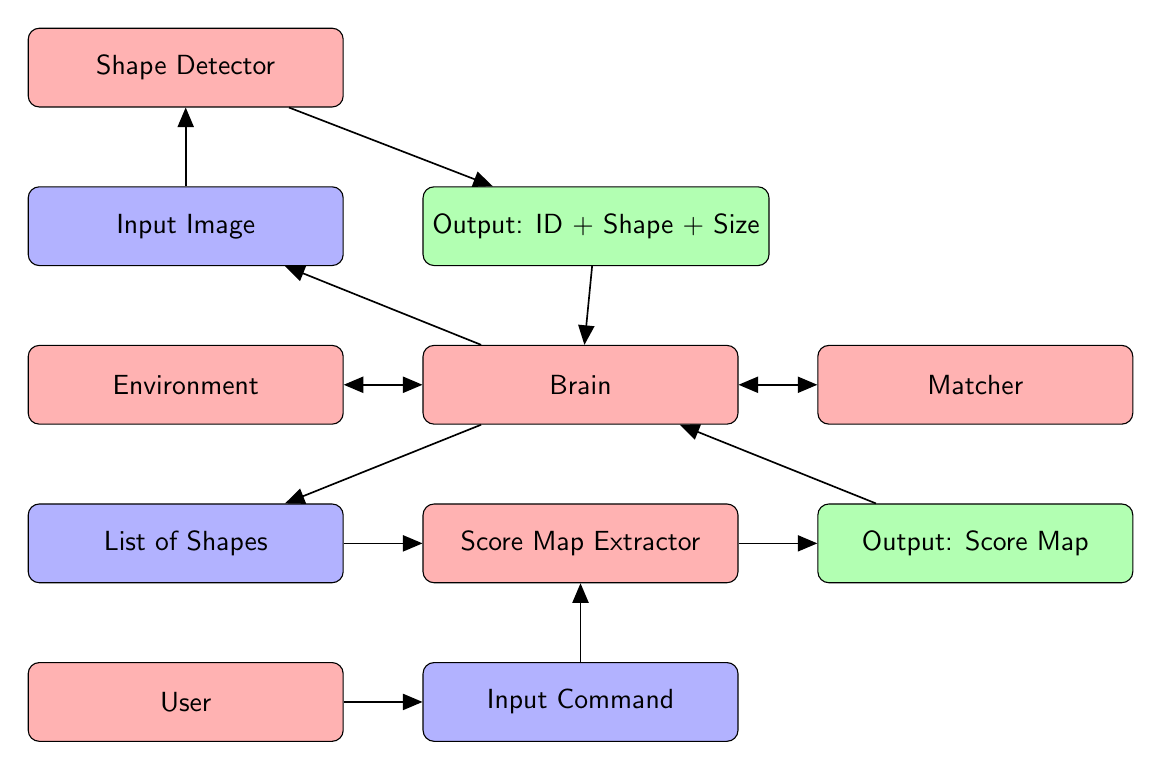
\begin{tikzpicture}[>=triangle 45,font=\sffamily]
		\node (Shape) [process]  {Shape Detector};
		\node (II)[input, below=1cm of Shape] {Input Image};
		
		\node (IO) [output,right =1cm of II]  {Output: ID + Shape + Size};
		
		\node (Env) [process, below = 1cm of II] {Environment};
		\node (Brain) [process,right=1cm of Env] {Brain};
		\node (List) [input, below = 1cm of Env] {List of Shapes};
		\node (User) [process, below =1cm of List] {User};
		
		
		\node (ScoreMap) [process,below =1cm of Brain]  {Score Map Extractor};
		\node (IC) [input,below =1cm of ScoreMap]  {Input Command};	
		\node (CO) [output,right =1cm of ScoreMap]  {Output: Score Map};
		
		\node (Matcher) [process, right=1cm of Brain] {Matcher};
		
		\draw [semithick,->] (II) -- (Shape);
		\draw [semithick,->] (Shape) -- (IO);
		
		\draw [semithick,->] (IO) -- (Brain);
		
		\draw [semithick,->] (IC) -- (ScoreMap);
		\draw [semithick,->] (ScoreMap) -- (CO);
		\draw [semithick,->] (CO) -- (Brain);
		
		\draw [semithick,<->] (Matcher) -- (Brain);
		
		\draw [semithick,<->] (Env) -- (Brain);
		\draw [semithick,->] (Brain) -- (II);
		\draw [semithick,->] (Brain) -- (List);
		\draw [semithick,->] (List) -- (ScoreMap);
		\draw [semithick,->] (User) -- (IC);
		
     \end{tikzpicture}
     
     \section{Architecture}
     The Architecture is composed of several parts that pass together to achieve the final Result or as i call it 'Action'.
     \subsection{Environemnt} The environment is a 3D world with different objects that is generated randomly on every test. The environment randomly selects 20 times from the set $\left\{ Cube, Sphere, Pyramid, Cylinder \right\}$ and for each objects it assigns a random size \textit{s} and color \textit{c}. These Objects are placed in the scene in such a way that they dont overlap with each other. The camera represents the robot which looks at this scene from a 45\textsuperscript{o} angle to mimic a situation where the robot is sitting on a table. A picture is taken of the scene at the time of evaluation. The picture is sent to the Brain which then calls the Shape Detector without giving him information about the number of objects or their shape.
     \subsection{Shape Detector}
     The Shape Detector is a model trained to recognize the basic shapes from the set $\left\{ , Sphere, Pyramid, Cylinder \right\}$ in an image taken from the environment. This module outputs an ID, a color, a size and a position for the all the shapes that it detects. The model is a trained End-to-End Modular Network(N2NMN) on the SHAPES Dataset.\\
     -TODO MORE INFO ON N2NMN\\
     It receives an image from the environment and then it asks several questions to the model about the image. The questions asked are the following:
     \begin{itemize}
     	\item How many Rectangular shapes are there in the image?
     	\item How many Sphere are there in the image?
     	\item How many Pyramids are there in the image?
     	\item How many Cylinders are there in the image?
     	\item What is the size of ...? (for every shape)
     	\item What is the color of ...? (for every shape)
     	\item Where is the ... placed (for every shape)
     \end{itemize}
 	 The results from this step are sent to the brain so that it has a list of all the objects in the image and their properties. Also the probability \textit{P(x)} for the best 3 possibilities for every property of every object is stored as well. If the Shape Detector says for a certain shape that it has a 50\% chance of being blue, 30\% chance of being green and maybe 20\% for yellow then all 3 results are stored with their probability.
     \subsection{Score Map Extractor}\
     The Score Map Extractor(SME) is called from the Brain to communicate with the user. The SME will first inquire about the action that it will take. The action can be \textit{select, move or remove}. Then it will ask for a description of the object and based on that it will return a score map which will be sent to the Brain. Last if the object has to be moved then it will ask the user for a description of the new location. This location will create a new score map which is also sent to the Brain.\\
     -TODO TEXTUAL GROUNDING USING IMAGE CONCEPTS\\
    
    \subsection{Brain}
    The Brain is the most important part of this architecture. Its first function is to control the flow of the operations and to make sure that each item fulfills its duties. It passes control to the Shape Detector and the Score Map Extractor so that they can complete their tasks and then collects all input and calls the Matcher to consult about the operation that it has to take. After it decides on what it should do then a command is sent to the Environment. The environment then responds by taking the action.
     
    
     \subsection{Matcher}
     The Matcher is called by the Brain to decide on the best action to take given the information it has. The matcher receives the list of objects with their properties and then uses the probabilities for every property of every object to decide on which object was most likely to be the one selected by the user. Then depending on the action verb that was selected and the Score Map of the new location it sends to the Brain a list of actions that can be taken and were the most likely to be what the user asked for. These can be several actions in that one could move an object that matches the color but not the shape while the second one can be the opposite. For example if the user says "Move the Red Square to the left" and there happens to be no Red Square but only a Red Cylinder and a Blue Square then both the actions that move these objects will be listed.
	
\end{document}
